\documentclass[11pt]{article}
\usepackage[T1]{fontenc}
\usepackage[margin=1in,top=0.6in,bottom=0.6in]{geometry}
\usepackage[bookmarks,colorlinks=true,linkcolor=blue,urlcolor=blue]{hyperref}
\usepackage{url}
\usepackage{tabularx}
\usepackage{graphicx}
\usepackage{placeins}
\usepackage{paralist}
\usepackage{makecell}
\usepackage[osf]{libertine}
\usepackage{zi4}
\usepackage[libertine,cmbraces]{newtxmath}

% configuration of source code examples
\usepackage{listings}
\lstset{language=c++}
\lstset{numbers=left}
\lstset{xleftmargin=2em}
\lstset{framexleftmargin=2em}
\lstset{belowskip=0em}
\lstset{belowcaptionskip=0em}
\lstset{tabsize=4}
\lstset{frame=single}
\lstset{breaklines=true}
\lstset{showspaces=false}
\lstset{showstringspaces=false}
\lstset{showtabs=false}
\lstset{breakatwhitespace=false}
\lstset{basicstyle=\small\ttfamily}

% table lines
\newcommand{\thinhline}{\Xhline{1\arrayrulewidth}}
\newcommand{\thickhline}{\Xhline{2.5\arrayrulewidth}}

\newcommand{\menustyle}[1]{\texttt{#1}}

\setcounter{tocdepth}{3}

\begin{document}

\title{glscopeclient Operator Manual}
\author{Andrew Zonenberg\\
azonenberg@drawersteak.com}
\date{\today}

\maketitle
\begin{abstract} \normalsize
This document is the user manual for glscopeclient, a user interface and signal analysis tool for oscilloscopes and
logic analyzers. As of this writing, glscopeclient is under active development but has not had a formal v0.1 release
and should be considered alpha quality.
\end{abstract}
\thispagestyle{empty}

\pagebreak

\tableofcontents

\pagebreak
\section{Revision History}
\begin{itemize}
\item \today: [in progress] Initial draft
\end{itemize}

\pagebreak
\section{Getting Started}

\subsection{Documentation Conventions}

Items to be selected from a menu are displayed in \menustyle{monospace font}.

Multilevel menu paths are separated by a / character. For example, \menustyle{Attenuation / 1x} means to open the
\menustyle{Attenuation} submenu and select the \menustyle{1x} item.

If there are multiple options for a menu or configuration option, they are displayed in square brackets and separated
by a | character. For example, \menustyle{Move waveform to / Waveform Group [1|2]} means to select either
\menustyle{Waveform Group 1} or \menustyle{Waveform Group 2} from the \menustyle{Move waveform to}
menu.

This project is under active development and is not anywhere near feature complete! As a result, this document is
likely to refer to active bug or feature request tickets on the GitHub issue trackers. Issues are referenced as
repository:ticket, for example scopehal-apps:3.

\subsection{Supported Hardware}

glscopeclient uses the libscopehal library to communicate with oscilloscopes, so any libscopehal-compatible hardware
should work with glscopeclient.

\begin{tabularx}{16cm}{lllllX}
\thickhline
Vendor & Device families & Driver & Tested on & Status \\
\thickhline
R\&S & RTM3000 & rs\_lan & (FIXME) & \makecell{Read-only mostly works\\can't change most settings} \\
\thickhline
Rigol & DS1000Z & rigol\_lan & DS1054Z & \makecell{Read-only mostly works\\can't change most settings} \\
\thickhline
Siglent & FIXME & lecroy\_lan & Untested & FIXME \\
\thickhline
Siglent & FIXME & lecroy\_vicp & Untested & FIXME \\
\thickhline
\makecell{Teledyne \\ LeCroy} & MAUI based & lecroy\_vicp & \makecell{WaveRunner 8104 \\ HDO9204} & Fully usable \\
\thickhline
\makecell{Teledyne \\ LeCroy} & T3DSO & lecroy\_lan & Untested & WIP \\
\thickhline
\end{tabularx}

\subsection{Compilation}

\begin{enumerate}

\item Install dependencies. On Debian/Ubuntu:
\begin{lstlisting}[language=sh]
sudo apt install build-essential cmake pkg-config libglm-dev \
	libgtkmm-3.0-dev libsigc++-2.0-dev
\end{lstlisting}

\item Install FFTS library
\begin{lstlisting}[language=sh]
git clone https://github.com/anthonix/ffts.git
cd ffts
mkdir build
cd build
cmake ../
sudo make install
\end{lstlisting}

\item Build scopehal and scopehal-apps
\begin{lstlisting}[language=sh]
git clone https://github.com/azonenberg/scopehal-cmake.git --recurse-submodules
cd scopehal-cmake
mkdir build
cd build
cmake ../
make
\end{lstlisting}

\item Install scopehal and scopehal-apps: right now, you don't. As of now, glscopeclient is intended to be run from the
glscopeclient binary directory (build/src/glscopeclient). Anybody want to contribute and set up a proper install
process?

\end{enumerate}

\subsection{Running glscopeclient}

There is not yet a proper GUI startup dialog for discovering and connecting to instruments. For the moment, you must
specify the instrument(s) you plan to connect to on the command line.

\begin{lstlisting}[language=sh]
./glscopeclient --debug \
	mylecroy:lecroy_vicp:myscope.example.com:1234 \
	myrigol:rigol_lan:rigol.example.com
\end{lstlisting}

The --debug argument may be omitted or replaced with any other liblogtools argument for controlling console debug
verbosity (--quiet, --verbose, --debug, --trace, etc). If you're using glscopeclient at its current level of maturity
you're probably a developer, so we suggest --debug.

Each instrument is described by a ``connection string" containing three colon-separated fields.

\begin{itemize}
\item Nickname. This can be any text string not containing spaces or colons. If you have only one instrument it's
largely ignored, but when multiple instruments are present channel names in the UI are prefixed with the nickname to
avoid ambiguity.
\item Driver name. This is a string identifying the command protocol and interface the scope uses. Note that not all
scopes from the same vendor will use the same command set or driver!
\item Arguments for the driver identifying the device to connect to, separated by colons. This varies by driver but is
typically a hostname:port combination, TTY device path, or similar.
\end{itemize}

\subsection{Design Philosophy}

glscopeclient's UI is heavily mouse driven and context based. Space used by always-visible buttons, sliders, etc is
kept to a minimum in order to keep as much screen real estate as possible usable for waveform display. Additional
controls are displayed in menus or pop-up dialogs, then hidden as soon as they are not needed.

Most UI elements can be interacted with by left clicking (select), left dragging (move), using the scroll wheel (zoom),
double clicking (open properties dialog), or right clicking (context menu).

\pagebreak
\section{Oscilloscope Drivers}

\subsection{Agilent}
TODO

\subsection{Antikernel Labs}
TODO

\subsection{Keysight}
TODO

\subsection{Rigol}
TODO

\subsection{Rohde \& Schwarz}
TODO

\subsection{Siglent}
TODO

\subsection{Teledyne LeCroy}
TODO

\subsection{Tektronix}
TODO

\pagebreak
\section{Main Window}

The main window of glscopeclient consists of the menu bar and tool bar at top and a status bar at the bottom. All
remaining space is occupied by one or more waveform groups.

\section{Waveform Groups}

A waveform group is a collection of one or more waveforms stacked vertically under a common timeline. All waveforms
within a group share the same timeline and vertical cursor(s).

When glscopeclient starts up, by default all channels on the attached instruments are displayed in a single waveform
group (Figure \ref{single-group}).

\begin{figure}[h]
\centering
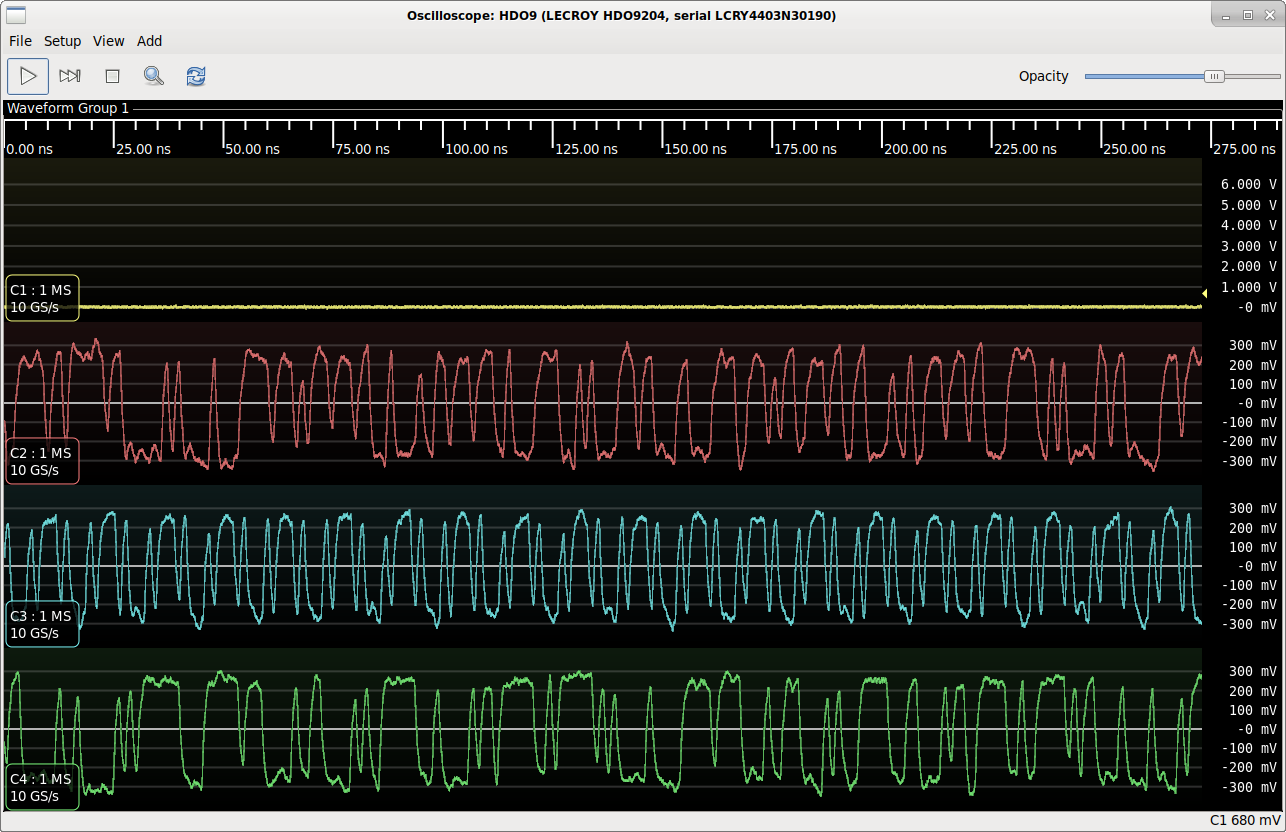
\includegraphics[width=13cm]{images/overview.png}
\caption{Top level glscopeclient window with a single waveform group}
\label{single-group}
\end{figure}

As you add protocol decodes or look at different parts of a waveform, it may be necessary to create additional waveform
groups. Typical reasons for creating additional groups include:

\begin{itemize}
\item Zooming into one set of signals to see detail on short time scales while maintaining a high level overview of
others
\item Viewing signals with incompatible horizontal units. For example, a FFT has horizontal units of frequency while an
analog waveform has horizontal units of time and eye patterns have horizontal units of UIs.
\footnote
{
It is currently possible to place signals with incompatible horizontal units in the same group. This may lead to
confusion; a future software release will likely force creation of a new group if a protocol decode is incompatible
with the parent trace's time scale.
}
\end{itemize}

\subsection{Managing Groups}

Additional groups may be created by right clicking a waveform and selecting \menustyle{[Move|Copy] waveform to / Insert
new group at [right|bottom]} from the context menu. This will split the current group's area in half horizontally or
vertically, with the selected waveform moved or copied to the newly added group and all other waveforms in the original
group.

Dividers between waveform groups may be dragged with the left mouse button. Any group may be subdivided again, to
create arbitrarily complex tiles of waveforms. Figure \ref{multiple-groups} shows a two-level hierarchy created by
moving channel 2 to a new group at right, moving channel 4 to this group, then moving channel 4 again a new group at
bottom.

\begin{figure}[h]
\centering
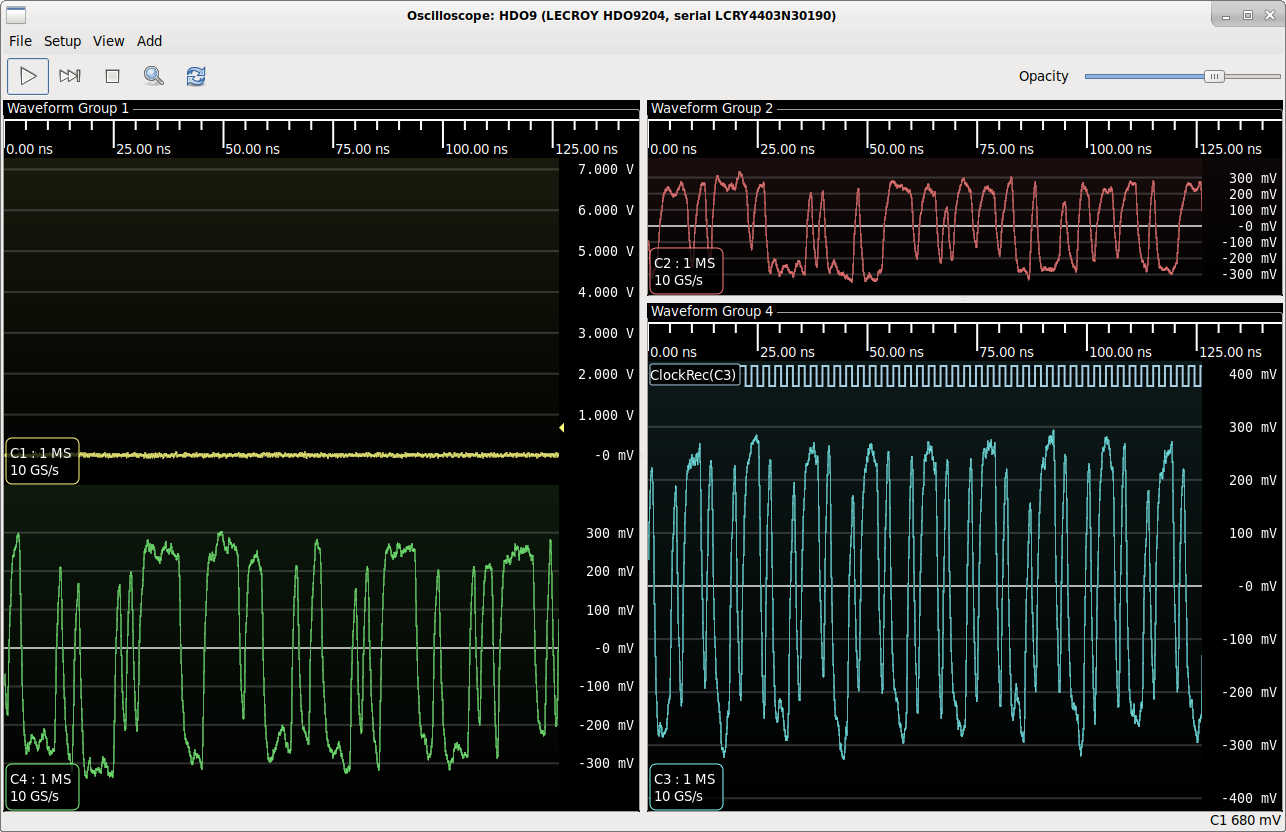
\includegraphics[width=14cm]{images/multiple-groups.png}
\caption{Top level glscopeclient window with several waveform groups separated by splitters}
\label{multiple-groups}
\end{figure}

A future software release will support using the mouse to move and copy waveforms, both between groups and within a
group (scopehal-apps:6). The exact semantics for this are not yet defined.

New waveform groups are given an automatically generated name when created, for example "Waveform Group 2". This name
will be editable in a future software release (scopehal-apps:53).

\section{Timeline}

The timeline is displayed at the top of each waveform group and shows the X axis scale for the group. The timeline (and
all accompanying waveform views in the group) may be zoomed by scrolling with the mouse wheel, or panned by dragging
with the left mouse button.

Unlike classical oscilloscope user interfaces, there is \emph{no relationship} between the timeline scale/position and
the duration of the acquisition. It is possible to zoom or scroll beyond the end of the acquisition (displaying empty
background with no signal) or have a deep capture in which nearly all acquired data is offscreen.

TODO: talk about how to set trigger offset in capture and change timebase once that's implemented

TODO: insert screenshot after we have some pending UI changes done

\section{Waveform Views}

A waveform view is a 2D graph of a signal or protocol decode within a waveform group.

\subsection{Graph}

\subsection{Y Axis}

Each waveform view has its own Y axis scale, which is locked to the ADC range of the instrument.

Dragging the Y axis scale with the left mouse button currently does nothing (scopehal-apps:54) but in a future software
release will change the voltage offset of the channel.

Scrolling the Y axis scale with the mouse wheel changes the gain of the channel.

\subsection{Channel Information Box}

The channel information box is displayed in the lower left corner of each waveform view. It contains summary
information about the channel. Currently this is the display name of the channel, the sample rate, and the record
length of the acquisition. Other information, such as probe coupling, may be displayed there in the future.

Double-clicking the information box opens the channel properties dialog.

\subsection{Overlays}

\section{Measurements}

\section{Protocol Decodes and Math Functions}

\subsection{Introduction}

\subsubsection{Key Concepts}

glscopeclient and libscopehal are based on a ``filter graph" architecture internally. The filter graph is a directed
acyclic graph with a set of source nodes (waveforms captured from hardware or loaded from a file) and sink nodes
(waveform views) connected by edges representing data flow.

A protocol decode is simply an intermediate node in the graph, which takes input from one or more waveform nodes and
outputs a waveform which may be displayed in a waveform view, used as input to other protocol decodes, or both. A
waveform is a series of data points which may represent voltages, digital samples, or arbitrarily complex protocol data
structures.

As a result, there is no internal distinction between math functions and protocol decodes, and it is possible to chain
them arbitrarily. Consider the following example\footnote{Not all of these filters are currently implemented}.

\begin{itemize}
\item Two analog waveforms representing serial data and clock are acquired
\item Each analog waveform is thresholded, producing a digital waveform
\item The two digital waveforms are decoded as $I^2C$, producing a series of packets
\item The $I^2C$ packets are decoded as writes to a serial DAC, producing an analog waveform
\item A moving average filter is applied to the analog waveform
\end{itemize}

In this document we use the term ``protocol decoder" consistently to avoid ambiguity.

\subsubsection{Conventions}

\subsection{8B/10B (IBM)}
\subsection{8B/10B (TMDS)}
\subsection{AC Couple}
\subsection{CAN}
\subsection{Clock Jitter (TIE)}
\subsection{Clock Recovery (PLL)}
\subsection{Clock Recovery Debug}
\subsection{Clock Recovery (UART)}
\subsection{DC Offset}
\subsection{Difference}
\subsection{DVI}
\subsection{Ethernet - 10baseT}
\subsection{Ethernet - 100baseTX}
\subsection{Ethernet Autonegotiation}
\subsection{Eye Pattern}
\subsection{FFT}
\subsection{$I^2C$}
\subsection{JTAG}
\subsection{MDIO}
\subsection{Moving Average}
\subsection{Period}
\subsection{Sin(x)/x Interpolation}
\subsection{Threshold}
\subsection{UART}
\subsection{USB 1.0 / 2.x Activity}
\subsection{USB 1.0 / 2.x Packet}
\subsection{USB 1.0 / 2.x PCS}
\subsection{USB 1.0 / 2.x PMA}
\subsection{Waterfall}

\end{document}
